\documentclass{article}
\usepackage{graphicx} % Required for inserting images
\usepackage{amssymb}
\usepackage{mathtools}
\usepackage{amsmath}
\graphicspath{{./images/}}

\makeatletter
\newcommand*{\rom}[1]{\expandafter\@slowromancap\romannumeral #1@}
\makeatother



\title{Midterm of DM}
\author{Swen Chan}
\date{June 2023}

\begin{document}

\maketitle

\section*{Question 1}

\section*{(a)}

\rom{1}:

\begin{figure}[h]
    \centering
    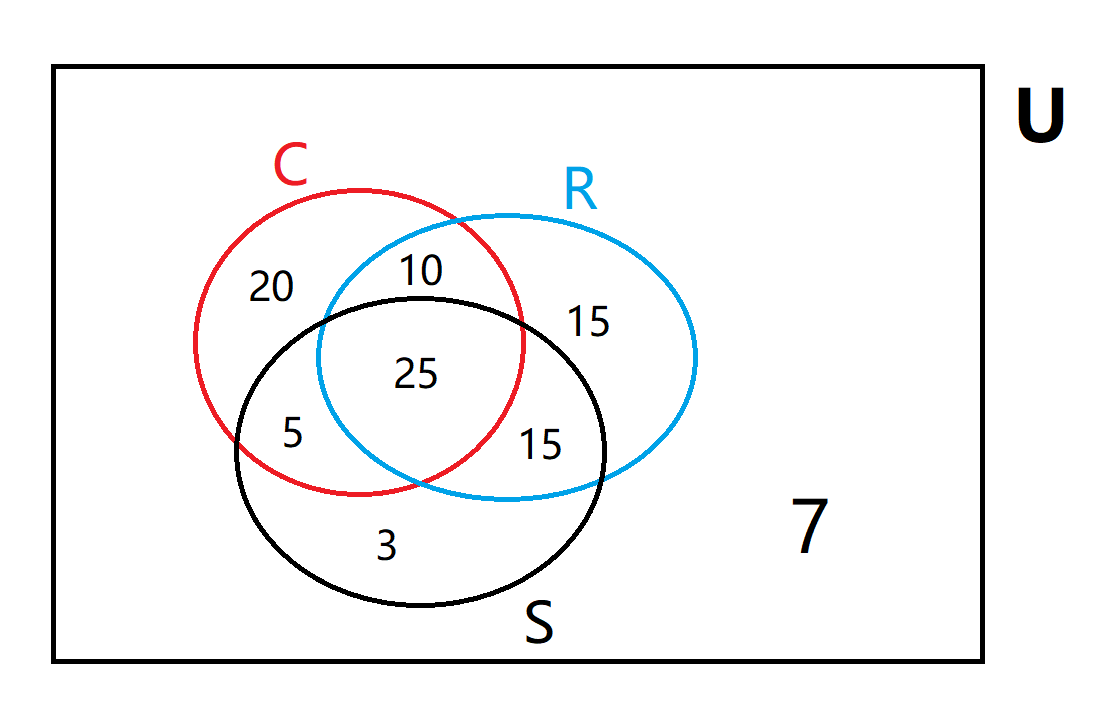
\includegraphics[width=0.75\textwidth]{Q1-1}
    \caption{Venn Gram}
    \label{fig:1}
\end{figure}

\rom{2}:
\(
|C \cup R \cup S| = |C| + |R| + |S| - |C \cap R| -|C \cap S| -|R \cap S| + |C \cap R \cap S|
\) 
= 93

\rom{3}:
\(|C \cup R \cup S|^\complement\) = 100 - 93 = 7

\rom{4}:
\(|C \oplus R \oplus S|=|C \cup R \cup S|-|C \cap R|-|C \cap S|-|R \cap S| + 2|C \cap R \cap S|\)=38

\rom{5}:
\(|C \oplus R|^\complement=100-(|C|+|R|-2|C\cap R|)\)=45

\section*{(b)}
1.i is False.\\
Counter-example:\\
A=\{1\}, B=\{2\}, P(A)=\{$\epsilon$,\{1\}\},P(B)=\{$\epsilon$,\{2\}\};\\
then \(A\cup B=\{1,2\},P(A\cup B)=\{\epsilon, \{1\}, \{2\}, \{1,2\}\}\\\{1,2\}\in P(A\cup B),but\{1,2\}\notin P(A)\cup P(B)\)\\so,i is FALSE.\\
\\
2.ii is True.\\
Proof1:\\
\(Assume:a \in A\cap B,so:a\in A,a\in B.\\Thus,a\in P(A\cap B),a\in P(A),a\in P(B).\)\\so,if 
\(\forall a,a\in P(A\cap B),\) such that  \(a\in P(A)\cap P(B)\\\)
\(so,P(A\cap B) \subseteq P(A)\cap P(B) \)\\
Proof2:\\
Assume:
\(a\in A,a\in B,then:a\in A\cap B.\)\\Thus,\(a\in P(A),a\in P(B),a \in P(A\cap B).\)\\
so,if \(\forall a,a\in P(A),a\in P(B)\),such that \(a\in P(A),a\in P(B)\)\\so,\(P(A)\cap P(B)\subseteq P(A\cap B)\)\\
\\From Proof1 and Proof2,we can conclude that \(P(A)\cap P(B) = P(A\cap B)\)

\section*{(c)}
Proof:\\
left=\((A\cup B^\complement)-B=(A\cup B^\complement)\cap B^\complement=(A\cap B^\complement)\cup (B^\complement\cap B^\complement)\\
=(A\cap B^\complement)\cup B^\complement)\\
=(A-B)\cup B^\complement\),which is right 


\section*{Question 2}

\section*{(a)}
i.
\(Domain_1=(-\infty,2),Range_1=R\\\)
ii.
\(Domain_2=[2/3,+\infty],Range_2=(-\infty,2]\\\)
iii.
\(Domain_3=R,Range_3=(1,+\infty)\)

\section*{(b)}
i.
\(f(x)=\frac{3(x+1)}{2x^2+7x-4}-\frac{1}{x+4}\\=\frac{3(x+1)}{(2x-1)(x+4)}-\frac{2x-1}{(2x-1)(x+4)}\\=\frac{x+4}{(2x-1)(x+4)}\\=\frac{1}{2x-1}(x>\frac{1}{2})\)\\
ii.
\(x=\frac{1}{2f^{-1}(x)}\longrightarrow f^{-1}(x)=\frac{1+x}{2x}\)\\
so \(f^{-1}:x\longrightarrow \frac{1+x}{2x},where>\frac{1}{2},and,x\in (0,+\infty)\)\\
iii.
\((fog(x)=f(log_{e}(x+1))=\frac{1}{2log_{e}(x+1)-1}=\frac{1}{7}\longrightarrow x=e^4-1\)

\section*{(c)}
i:F is not a one-to-one function.\\
Counter-example:\\
\(m=\{0,1\}\in P(\{a,b,c\})\\n=\{1,2\}\in P(\{a,b,c\})\\m\ne n,but,F(m)=F(n)=2\)
,so,F is not a one-to-one function.\\
ii.F is an onto function.\\
\(Co-domain=\{0,1,2,3,4\}\\\)since for all \(y\in Co-domain,\)there exists \(x\in P(\{a,b,c\}),\)such that \(F(x)=y\)\\Thus,F is an onto function.

\section*{(d)}
Assume that \(gof\) is onto.\\
for any \(c\in C\),there exists \(a\in A\),such that \(gof(a)=c\)\\so for any \(c\in C\),there exists \(f(a)=b\),such that \(g(b)=c\)\\And \(b\in B\).Thus,for any \(c\in C\),there exists \(b\in B\),and \(b=f(a)\),such that \(g(b)=c\)\\
so g is also onto.

\section*{Question 3}

\section*{(a)}
i.\(((p\land \lnot q)\longrightarrow(q\land r))\longrightarrow (s\lor \lnot q)\)is True.\\
\(q\land s\) is True,so q is True and s is True.\\
Then \(s\lor\ \lnot q\) is True, \(p\land \lnot q\) is False.\\ \(p\land \lnot q\) is False\(\longrightarrow (p\land \lnot q)\longrightarrow (q\land r)\) is True.\\since \(s \lor \lnot q\) is True,\\
\(((p\land \lnot q)\longrightarrow (q\land r))\longrightarrow (s\lor \lnot q)\)is True.\\
ii.\(q\lor s\) is True,so \(((p\lor q)\land (q\lor s))\longrightarrow ((\lnot r\lor p)\land (q\lor s))\Longleftrightarrow(p\lor q)\longrightarrow (\lnot r\lor p)\)\\
q is Ture,so \(p\lor q\) is True.\\since \(p\lor r\) is False,\(\lnot r \lor p\) is not certain:\\
If r is False,p is True,then \(\lnot r \lor p\)  is True.\\Then \((p\lor q)\longrightarrow (\lnot r \lor p)\) is True.\\But if \(r\) is True,\(p\) is False,then \(\lnot r \lor p\) is False.\\
Then \((p\lor q)\longrightarrow (\lnot \lor p)\) is False.\\So the value of \(((p\lor q)\land (q\lor s))\longrightarrow ((\lnot r\lor p)\land (q\lor s))\) is not sure.

\section*{(b)}
i.\(h\land w\land \lnot s\)\\
ii.\(\lnot h\land \lnot w\land s\)\\
iii.\(h\oplus w\)

\section*{(c)}
i.\\Contrapositive:\(\forall x\in R\),if \(x^2\le 4\),then \(x < 2\)\\
Converse:\(\forall x\in R\),if \(x^2 > 4\), then \(x > 2\)\\
Inverse:\(\forall x\in R\),if \(x\le 2\),then \(x^2\le 4\) \\
ii.\\Contrapositive:\(\forall x\in R\),if \(-2\le x\le 0\),then \(x(x+2)\le 0\)\\
Converse:\(\forall x\in R\), if \(x>0\) or \(x<-2\),then \(x(x+2))>0\)\\
Inverse:\(\forall x\in R\),if \(x(x+2)\le 0\),then \(-2\le x\le 0\)\\

\section*{(d)}
Proof:\\
\((p\longrightarrow (q \lor v))\Longleftrightarrow \lnot p \lor(q\lor r)\Longleftrightarrow \lnot p \lor q \lor r\Longleftrightarrow(\lnot p\lor q)\lor r\Longleftrightarrow \lnot(p\land \lnot q)\lor r\Longleftrightarrow(p\land \lnot q)\longrightarrow r\)\\
\section*{Question 4}

\section*{(a)}
i is False.\\Counter-example:\\Assume \(x=1\),since \(x=y+1,y=0\).but 0 \(\notin Z^{+}.\)\\\\
ii is True.\\Proof:for \(\forall y\in Z^+,\exists x=y+1\),such that \(x=y+1.\)\\
since \(y\in Z^+\), \(y+1\in Z^+\).\\\\
iii is True.\\Proof:Each pair of \((x,y)\)which \(x\) is 1 larger than \(y\),can get \(x=y+1\).\\
So there are many possibilities to satisfy the demand.

\section*{(b)}
i."The football game will be cancelled only if it rains."\(\Longleftrightarrow q\longrightarrow p.\)\\
"It rained,therefore the football game was cancelled."\(\Longleftrightarrow p\longrightarrow q.\)\\
ii.
\begin{center}
\begin{tabular}{ c c c c}
 p & q & \(p\longrightarrow q\) & \(q\longrightarrow p\) \\ 
 F & F & T & T\\  
 F & T & T & F\\
 T & F & F & T\\
 T & T & T & T\\    
\end{tabular}
\end{center}

iii.\\
The first argument"The football game will be cancelled only if it rains."is not valid.\\
The second argument"It rained,therefore the football game was cancelled."is valid.\\

\section*{(c)}
if (a)(b)(c)are true,it's possible that Johnny does have five years of work experience.So this argument is not valid.
\section*{(d)}
In i,they haven't the same truth value for every choice of P(x),Q(x)and D.\\
In ii,they have the same truth table for every choice of P(x),Q(x) and D.\\


\section*{Question 5}

\section*{(a)}
i.\((ab)^\complement(a^\complement+b)(b^\complement+b)\\=(ab)^\complement(a^\complement+b)\\
=(ab)^\complement.a^\complement+(ab)^\complement.b\\=(a^\complement+b^\complement).a^\complement+(a^\complement+b^\complement).b\\=a^\complement+a^\complement.b^\complement+a^\complement.b+0\\
=a^\complement+a^\complement(b^\complement+b)\\=a^\complement+a^\complement\\=a^\complement\)\\
\\
ii.\(a^\complement(a+b)+(b+aa)(a+b^\complement)\\=a^\complement a+a^\complement b+ba+aaa+bb^\complement+aab^\complement\\=a^\complement b+ba+a+ab^\complement\\=b(a+a^\complement)+a(a+b^\complement)\\=b+a+ab^\complement\)
\section*{(b)}
Use the duality principle:\\
left=\(ab+cd^\complement=(a+b)(c+d^\complement)=ac+ad^\complement+bc+bd^\complement\\=(a+c)(a+d^\complement)(b+c)(b+d^\complement)\)=right
\section*{(c)}
i.Truth table:\\
\begin{center}
\begin{tabular}{ c c c }
 x & y & \(F(x,y)\) \\ 
 1 & 1 & 0 \\  
 1 & 0 & 1 \\
 0 & 1 & 1 \\
 0 & 0 & 0 \\    
\end{tabular}
\end{center}

ii.
F(x,y) = 
\[ 
\begin{cases} 
      0, & \textit{x is the same as y} \\
      1, & \textit{x is different from y}\\ 
   \end{cases}
\]

iii.
\begin{figure}[h]
    \centering
    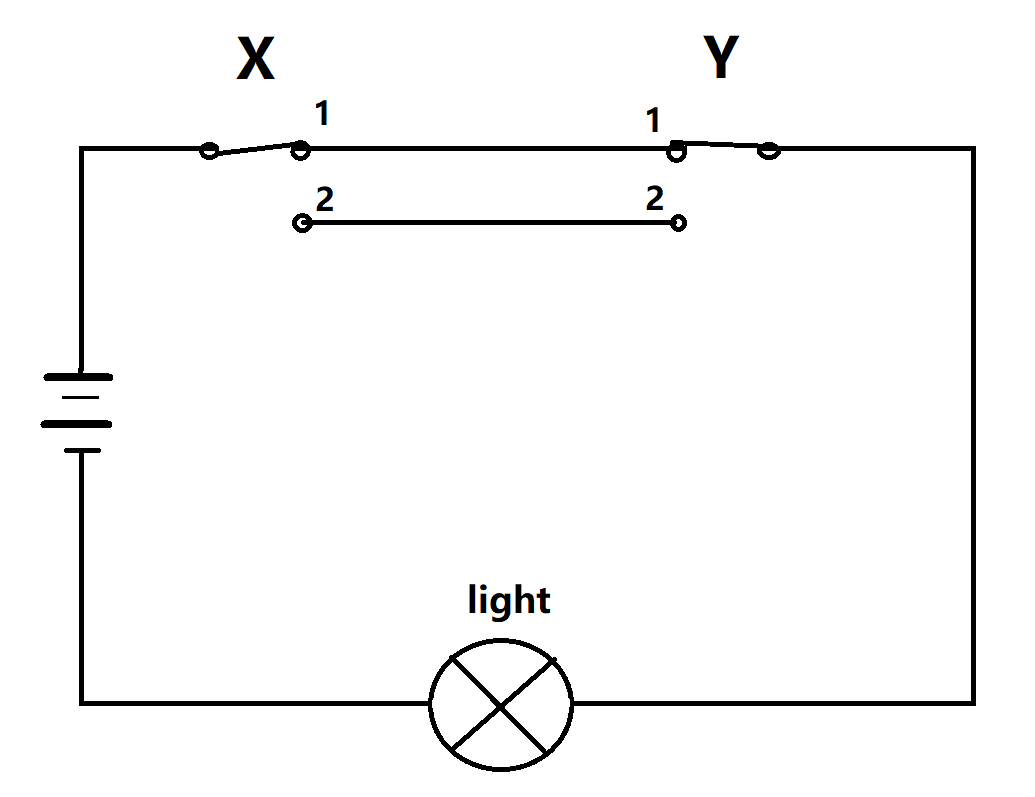
\includegraphics[width=0.75\textwidth]{Q5}
    \caption{circuit}
    \label{fig:1}
\end{figure}
\section*{(d)}
i.
K-map for F(A,B,C,D):
\begin{center}
\begin{tabular}{ c c c c c }
  & \(AB\) & \(A^\complement B\) & \(AB^\complement\) & \((AB)^\complement\) \\ 
 \(CD\)                & 1 & 1 & 1 & 1\\  
 \(C^\complement D\)   & 1 & 0 & 0 & 0 \\
 \(CD^\complement)\)   & 1 & 0 & 0 & 0 \\
 \((CD)^\complement\)  & 1 & 0 & 0 & 0 \\    
\end{tabular}
\end{center}
ii.minimisation of \(F(A,B,C,D)=AB+CD\)
\end{document}


